\section{Setup}
\label{sec:setup}

In the following, the setup is explained. 

The measurement setup comprises a broad-spectrum lamp and a UV-Vis spectrometer situated at the end of a light guide. This setup can be used for both reflectance and transmission measurements. To measure reflectance, a fiber with three ends is used, with inputs for the lamp and outputs for both the UV-Vis and NIR spectrometers (see Figure \ref{fig:setup}). On the other end of the fiber, there is a combination of input and output ends. The single end is positioned in the sample holder, with the sample placed at approximately \SI{1}{\centi\metre} below sample holder.

\begin{figure}[ht]
    \centering
    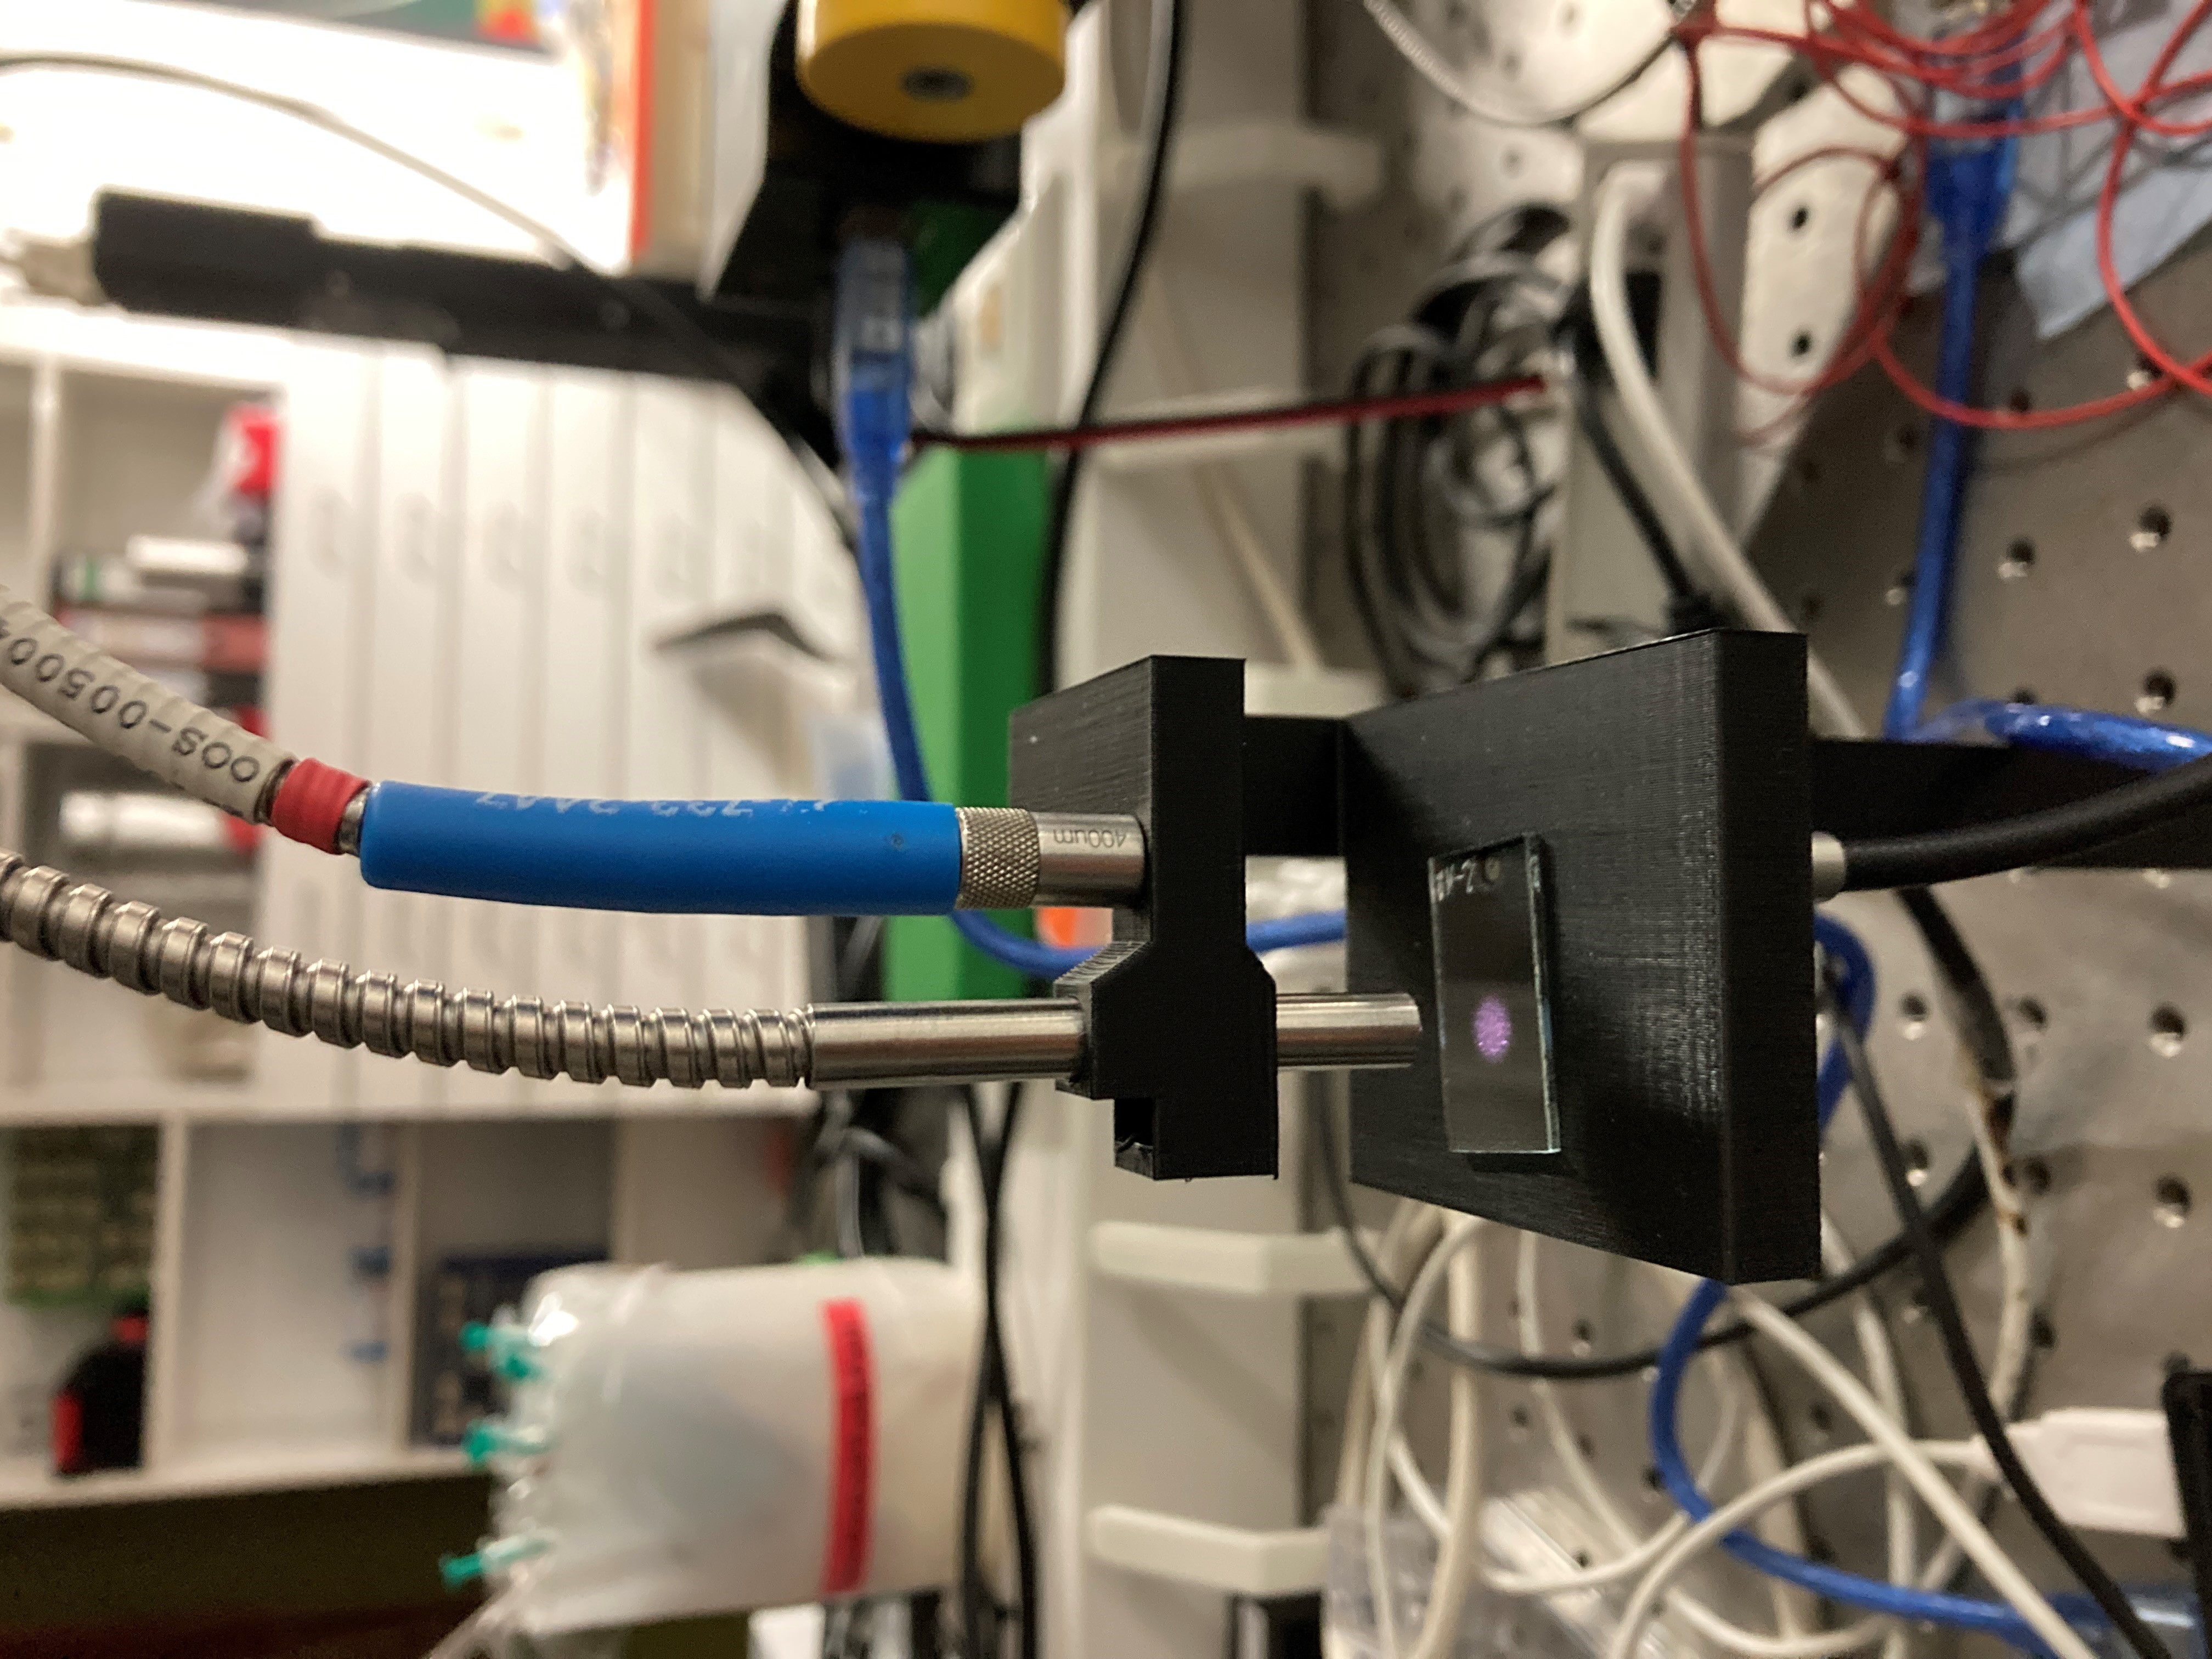
\includegraphics[width = 10cm, angle = -90]{Bilder/Auswertung/Setup/Setup.jpg}
    \caption{Sample holder with optic fiber and film}
    \label{fig:setup}
\end{figure}

Before conducting each series of film measurements, we capture a white spectrum of the lamp without any film. This data is then used by the program \textit{Nanocalc} to calculate the absorbance. At the start of each series, we measure the background once. Subsequently, we measure the spectrum of each film at six randomly selected points.